\documentclass[12pt,letterpaper, onecolumn]{exam}
\usepackage{amsmath}
\usepackage{amssymb}
\usepackage{amsfonts}
\usepackage{graphicx}
\usepackage{subcaption}
\usepackage{float}
\usepackage[shortlabels]{enumitem}
\usepackage{mathtools}
\usepackage{longtable}
\usepackage{tikz}
\usetikzlibrary{decorations.pathreplacing}

\usepackage[lmargin=71pt, tmargin=1.2in]{geometry} %For centering solution box
\lhead{STAT 8305 - Homework 2\\}
\rhead{Tommy Stell\\}
% \chead{\hline} % Un-comment to draw line below header
\thispagestyle{empty}   %For removing header/footer from page 1

\begin{document}

\begingroup
    \centering
    \LARGE Pattern Recognition\\
    \LARGE Homework 2\\[0.5em]
    \large \today\\[0.5em]
    \large Tommy Stell\par

\endgroup
\noindent\rule{\textwidth}{0.4pt}
\pointsdroppedatright   %Self-explanatory
\printanswers
\renewcommand{\solutiontitle}{\noindent\textbf{Ans:}\enspace}   %Replace "Ans:" with starting keyword in solution box

\begin{questions}

    \question Cross-Validation for Dependent Data

    Suppose we observe a dataset
    \begin{equation*}
        D_n = \{(X_i, Y_i) : i = 1,\dots,n\},
    \end{equation*}
    where $X_i$ and $Y_i$ denote the input and output, respectively. Assume that a prediction model is available and can be fitted using all or part of the data. Once fitted, the model produces predicted values $\hat Y_i$ for the corresponding inputs $X_i$.

    Design a cross-validation procedure for evaluating prediction performance when observations are dependent. You may consider temporal, spatial, grouped, or another appropriate dependence structure.
    \begin{enumerate}[(a)]
        \item Dependence assumptions. Describe a possible dependence structure among the observations. Clearly state your assumptions and, if appropriate, specify a correlation model with sufficient parameters to characterize the dependence.
        \item Data splitting. Explain how you would divide the data into training and validation sets. Clearly define which observations are used for model fitting and which are used for evaluating predictions.
        \item Cross-validation formula. Define an appropriate prediction loss function $L(Y_i,\hat Y_i)$ and write down the mathematical formula for the CV error under your proposed splitting procedure. Clearly define all notation used in the formula.
        \item Justification. Explain why your splitting strategy is appropriate under your dependence assumptions. In particular, discuss how it avoids information leakage, reduces problematic dependence between training and validation observations when necessary, and provides a meaningful evaluation of prediction performance.
    \end{enumerate}

    \newpage
    \begin{solution}

        I will work with temporal dependence. A concrete example to keep in mind is daily electricity demand $Y_i$ for a city, with inputs $X_i$ such as temperature, day of the week and holiday indicators. Demand on day $i$ is not only driven by $X_i$. Unmeasured things like a local event or a slow change in economic activity push demand up or down for several days in a row, so the errors on nearby days are correlated.

        \begin{enumerate}[(a)]
            \item Dependence assumptions. I assume the following.
            \begin{enumerate}[(A1)]
                \item The index $i$ is time. The observations are equally spaced and in time order, so $|i-j|$ is the time lag between observations $i$ and $j$.
                \item The output follows a regression model with additive error,
                \begin{equation*}
                    Y_i = f(X_i) + \varepsilon_i, \qquad E[\varepsilon_i]=0,
                \end{equation*}
                where $f$ is the unknown regression function the prediction model is trying to learn.
                \item The inputs are exogenous, i.e.\ $\{X_i\}$ is independent of $\{\varepsilon_i\}$, and I treat the $X_i$ as fixed when computing moments. The inputs can be autocorrelated themselves (temperature on consecutive days is similar), and that is allowed.
                \item The errors are a stationary first-order autoregressive, AR(1), process,
                \begin{equation*}
                    \varepsilon_i = \rho\,\varepsilon_{i-1} + \eta_i, \qquad \eta_i \overset{\text{iid}}{\sim} (0,\ \sigma^2(1-\rho^2)), \qquad |\rho|<1,
                \end{equation*}
                where $\eta_i$ is independent of $\varepsilon_{i-1},\varepsilon_{i-2},\dots$
            \end{enumerate}
            Under (A4) the innovation variance is chosen so that $\operatorname{Var}(\varepsilon_i) = \sigma^2(1-\rho^2)/(1-\rho^2) = \sigma^2$ for every $i$, and
            \begin{equation*}
                \operatorname{Cov}(\varepsilon_i,\varepsilon_j) = \sigma^2\rho^{|i-j|}, \qquad \operatorname{Corr}(\varepsilon_i,\varepsilon_j) = \rho^{|i-j|}.
            \end{equation*}
            The dependence is fully described by two parameters. $\sigma^2$ is the marginal error variance, and $\rho$ is the lag-1 correlation, which also sets how fast the correlation dies off with lag. For example, with $\rho = 0.8$ the correlation is $0.8$ at lag 1, $0.8^{7}\approx 0.21$ at lag 7 and $0.8^{14}\approx 0.044$ at lag 14.

            In practice, $\rho$ can be estimated from the residuals $\hat\varepsilon_i = Y_i - \hat f(X_i)$ of a rigid pilot fit (e.g.\ linear in $X$) by the lag-1 sample autocorrelation
            \begin{equation*}
                \hat\rho = \frac{\sum_{i=2}^{n}\hat\varepsilon_i\hat\varepsilon_{i-1}}{\sum_{i=1}^{n}\hat\varepsilon_i^{\,2}}.
            \end{equation*}
            The pilot should be rigid because a flexible fit absorbs part of the autocorrelation into $\hat f$, which pulls $\hat\rho$ toward zero and would make the buffer too small. $\hat\rho$ is only used to set the buffer width in (b). It never enters the fitted prediction model. The AR(1) model is a working assumption. If the residual autocorrelation function decays more slowly than $\hat\rho^{\,\ell}$, the only change to the procedure below is that the buffer width is read off the autocorrelation function directly instead of from $\rho$.

            Prediction target. What I want to evaluate is how well $\hat f$ has learned the relationship between $X$ and $Y$. That means the expected loss on a new observation from a stretch of time the model has not seen, whose error $\varepsilon$ is (nearly) uncorrelated with the errors the model was fit on. An example is fitting on past years and predicting demand for a new period from its temperatures and calendar. This target decides the split in part (b). If the goal were instead short-horizon forecasting, a forward-chaining split would be the right one, and I give it as a variant at the end of (b).

            \item Data splitting. I use blocked $K$-fold CV with a buffer. This extends the $h$-block idea of Burman, Chow and Nolan (1994), which leaves out one point at a time together with $h$ neighbors on each side, to validation blocks of length $b$ (their $h$ is my $m$). There are three steps.
            \begin{enumerate}[1.)]
                \item Cut the time axis into $K$ contiguous blocks of length $b = \lfloor n/K\rfloor$,
                \begin{align*}
                    V_k &= \{(k-1)b+1,\ \dots,\ kb\}, \qquad k=1,\dots,K-1,\\
                    V_K &= \{(K-1)b+1,\ \dots,\ n\},
                \end{align*}
                so the last block takes the remainder when $K$ doesn't divide $n$.
                The blocks don't overlap and together they cover $\{1,\dots,n\}$, so every observation is validated exactly once.
                \item Choose a buffer width $m\ge 0$. Observations within $m$ time steps of the validation block are thrown away for that fold. They are used neither for fitting nor for validation,
                \begin{align*}
                    G_k &= \{\,j\notin V_k : \min_{i\in V_k}|i-j| \le m\,\}\\
                    &= \{(k-1)b+1-m,\ \dots,\ (k-1)b\}\ \cup\ \{kb+1,\ \dots,\ kb+m\},
                \end{align*}
                intersected with $\{1,\dots,n\}$ (for $k=K$ the block ends at $n$), so the first and last blocks only have a buffer on one side.
                \item The training set is everything else,
                \begin{equation*}
                    T_k = \{1,\dots,n\}\setminus (V_k\cup G_k) = \{\,j : \min_{i\in V_k}|i-j| > m\,\}.
                \end{equation*}
            \end{enumerate}
            For fold $k$, the model is fit on $\{(X_j,Y_j): j\in T_k\}$ only, and it is evaluated on $\{(X_i,Y_i): i\in V_k\}$. The layout for an interior fold is,
            \begin{center}
                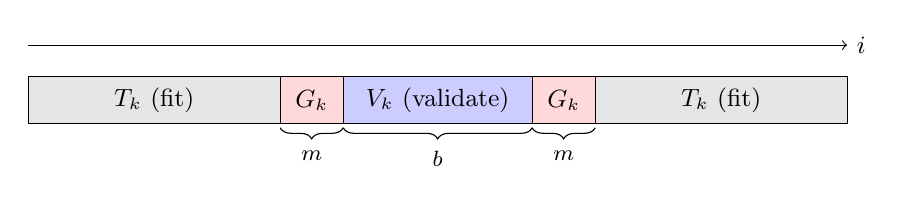
\begin{tikzpicture}[x=0.8cm, y=1cm]
                    \fill[gray!20] (0,0) rectangle (4,0.6);
                    \fill[red!15] (4,0) rectangle (5,0.6);
                    \fill[blue!20] (5,0) rectangle (8,0.6);
                    \fill[red!15] (8,0) rectangle (9,0.6);
                    \fill[gray!20] (9,0) rectangle (13,0.6);
                    \draw (0,0) rectangle (13,0.6);
                    \foreach \x in {4,5,8,9} \draw (\x,0) -- (\x,0.6);
                    \node at (2,0.3) {\small $T_k$ (fit)};
                    \node at (4.5,0.3) {\small $G_k$};
                    \node at (6.5,0.3) {\small $V_k$ (validate)};
                    \node at (8.5,0.3) {\small $G_k$};
                    \node at (11,0.3) {\small $T_k$ (fit)};
                    \draw[decorate, decoration={brace, mirror, amplitude=4pt}] (4,-0.05) -- (5,-0.05) node[midway, below=5pt] {\footnotesize $m$};
                    \draw[decorate, decoration={brace, mirror, amplitude=4pt}] (5,-0.05) -- (8,-0.05) node[midway, below=5pt] {\footnotesize $b$};
                    \draw[decorate, decoration={brace, mirror, amplitude=4pt}] (8,-0.05) -- (9,-0.05) node[midway, below=5pt] {\footnotesize $m$};
                    \draw[->] (0,1.0) -- (13,1.0) node[right] {\small $i$};
                \end{tikzpicture}
            \end{center}

            Choosing $m$. The closest a training point can be to a validation point is lag $m+1$, so under (A4) every training error has
            \begin{equation*}
                |\operatorname{Corr}(\varepsilon_i,\varepsilon_j)| = |\rho|^{|i-j|} \le |\rho|^{m+1}, \qquad i\in V_k,\ j\in T_k.
            \end{equation*}
            I pick a tolerance $c$ for how much correlation is acceptable (e.g.\ $c=0.05$; this is a choice, not something the model gives us) and take the smallest $m$ with $|\rho|^{m+1}\le c$,
            \begin{equation*}
                m = \left\lceil \frac{\ln c}{\ln|\rho|}\right\rceil - 1, \qquad 0<|\rho|<1,
            \end{equation*}
            with $m=0$ when $\rho=0$. For $\rho = 0.8$ and $c = 0.05$, $\ln 0.05/\ln 0.8 = (-2.9957)/(-0.2231) \approx 13.43$, so $m = 14-1 = 13$. As a check, $0.8^{14}\approx 0.044\le 0.05$, while $m=12$ would give $0.8^{13}\approx 0.055 > 0.05$.

            Two practical requirements go with this. First, the block length should be much larger than the buffer, $b \gg 2m$, so that each fold still has most of the data for fitting. For example, with $n = 1000$ and $K = 10$, $b = 100$ and an interior fold trains on $1000-100-2(13) = 874$ observations. Second, if the inputs contain lagged outputs (e.g.\ $X_j$ includes $Y_{j-1},\dots,Y_{j-p}$), then a training row just after the block would carry validation outputs inside its inputs. In that case the buffer after $V_k$ has to be widened from $m$ to $m+p$, so that no index used by a training row, as an input or as an output, is within $m$ of the block. Lagged outputs break (A3), though, since $Y_{i-1}$ has correlation $\rho$ with $\varepsilon_i$, so the leakage bound in (d) no longer applies. A model like that is really a forecasting model, and it belongs with the forward variant below. For the main procedure I keep the inputs exogenous, as in (A3).

            Variant for forecasting. If the goal is to forecast $h\ge 1$ steps past the end of the data we have, the split should only ever train on the past. With an initial training length $n_0$ and block length $v$, fold $k$ uses
            \begin{equation*}
                T_k = \{1,\dots,t_k\}, \qquad V_k = \{t_k+h,\ \dots,\ t_k+h+v-1\}, \qquad t_k = n_0+(k-1)v,
            \end{equation*}
            for $k=1,\dots,K$ with $K = \lfloor (n-n_0-h+1)/v\rfloor$, so that the last block ends at or before $n$. The gap $\{t_k+1,\dots,t_k+h-1\}$ is the forecast horizon, not a decorrelation buffer.

            \item Cross-validation formula. I use squared error loss,
            \begin{equation*}
                L(Y_i,\hat Y_i) = (Y_i-\hat Y_i)^2,
            \end{equation*}
            which matches the regression model in (a), since $E[(Y_i-\hat Y_i)^2]$ splits into the error variance $\sigma^2$ plus the error of $\hat f$ (see (d)). If a few large errors shouldn't dominate, absolute error $|Y_i - \hat Y_i|$ can be used in the same formulas.

            Let $\hat f^{(-k)}$ be the model fit on $\{(X_j,Y_j): j\in T_k\}$ only. This includes every data-dependent step: centering and scaling of the inputs, feature selection and hyperparameter tuning all use $T_k$ alone. The prediction for a validation point is $\hat Y_i^{(-k)} = \hat f^{(-k)}(X_i)$ for $i\in V_k$. The error on fold $k$ is
            \begin{equation*}
                \text{CV}_k = \frac{1}{|V_k|}\sum_{i\in V_k} L\bigl(Y_i,\ \hat f^{(-k)}(X_i)\bigr),
            \end{equation*}
            and since the blocks $V_1,\dots,V_K$ partition $\{1,\dots,n\}$, the blocked-buffered CV error is
            \begin{equation*}
                \text{CV}_{K,m} = \frac{1}{n}\sum_{k=1}^{K}\sum_{i\in V_k}\Bigl(Y_i-\hat f^{(-k)}(X_i)\Bigr)^2 = \sum_{k=1}^{K}\frac{|V_k|}{n}\,\text{CV}_k,
            \end{equation*}
            where
            \begin{itemize}
                \item $n$ is the number of observations and $K$ is the number of blocks (folds),
                \item $V_k$ is the $k$-th contiguous validation block, with length $|V_k| = b = \lfloor n/K\rfloor$ for $k<K$ and $|V_K| = n-(K-1)b$,
                \item $m$ is the buffer width from (b), and $G_k$ the buffer indices that are dropped from fold $k$,
                \item $T_k = \{j : \min_{i\in V_k}|i-j|>m\}$ is the training set of fold $k$,
                \item $\hat f^{(-k)}$ is the model fit on $T_k$, and $\hat Y_i^{(-k)} = \hat f^{(-k)}(X_i)$ is its prediction for $i\in V_k$.
            \end{itemize}
            With $m=0$ this is plain blocked $K$-fold CV, and with $m=0$ and the blocks replaced by random subsets it is ordinary $K$-fold CV.

            For the forecasting variant, the first $n_0+h-1$ observations are never validated, so the average has to be taken over the validated points rather than over $n$,
            \begin{align*}
                \text{CV}_{\text{fwd}} &= \frac{1}{\sum_{k=1}^{K}|V_k|}\sum_{k=1}^{K}\sum_{i\in V_k}\Bigl(Y_i-\hat f^{(-k)}(X_i)\Bigr)^2\\
                &= \frac{1}{Kv}\sum_{k=1}^{K}\sum_{i=t_k+h}^{t_k+h+v-1}\Bigl(Y_i-\hat f^{(-k)}(X_i)\Bigr)^2,
            \end{align*}
            where $\hat f^{(-k)}$ is fit on $\{1,\dots,t_k\}$.

            \item Justification. The problem with random $K$-fold CV here comes from one term. Write $D_i = \hat f^{(-k)}(X_i) - f(X_i)$ for the error of the fitted function at a validation point. Then $Y_i - \hat Y_i = \varepsilon_i - D_i$, and
            \begin{equation*}
                E\bigl[(Y_i-\hat Y_i)^2\bigr] = \sigma^2 + E\bigl[D_i^2\bigr] - 2\,E\bigl[\varepsilon_i D_i\bigr].
            \end{equation*}
            For a new observation whose error is independent of the training data, $E[\varepsilon_i D_i] = 0$, and the expected loss is $\sigma^2 + E[D_i^2]$. That is the quantity I said in (a) I want to estimate. When $\varepsilon_i$ is correlated with the training errors, $\hat f^{(-k)}$ has partly fit $\varepsilon_i$ through its neighbors, so $E[\varepsilon_i D_i]>0$ and the CV error comes out too small. This is the information leakage.

            To see how big the cross term can be, take a linear smoother, $\hat f^{(-k)}(X_i) = \sum_{j\in T_k} s_{ij}Y_j$, where the weights $s_{ij}$ depend only on the inputs. This covers least squares, ridge, splines, kernel regression and $k$-nearest neighbors. Using (A3),
            \begin{equation*}
                E\bigl[\varepsilon_i D_i\bigr] = \sum_{j\in T_k} s_{ij}\,E[\varepsilon_i\varepsilon_j] = \sigma^2\sum_{j\in T_k} s_{ij}\,\rho^{|i-j|}.
            \end{equation*}
            Under my split every $j\in T_k$ has $|i-j|\ge m+1$, so
            \begin{equation*}
                \bigl|E[\varepsilon_i D_i]\bigr| \le \sigma^2|\rho|^{m+1}\sum_{j\in T_k}|s_{ij}| \le c\,\sigma^2\sum_{j\in T_k}|s_{ij}|.
            \end{equation*}
            For an averaging smoother (nonnegative weights that add up to 1, like $k$-nearest neighbors or a kernel average) the sum is 1, so the bias from leakage in each validation term is at most $2c\sigma^2$, i.e.\ $0.1\sigma^2$ for $c=0.05$. The buffer is what turns the tolerance $c$ into a bound on the leakage.

            A worst-case example. Suppose the inputs include the time index, so that the learner is 1-nearest neighbor in time and $\hat f(X_i) = Y_j$ for the closest training time $j$. Take $f$ to be roughly constant over the lags involved, so $D_i \approx \varepsilon_j$. Then
            \begin{equation*}
                E\bigl[(Y_i-\hat Y_i)^2\bigr] \approx E\bigl[(\varepsilon_i-\varepsilon_j)^2\bigr] = 2\sigma^2\bigl(1-\rho^{|i-j|}\bigr).
            \end{equation*}
            For a truly new observation, this learner's error is $2\sigma^2$. Under random 10-fold CV, a neighbor at lag 1 is almost always in training, so with $\rho = 0.8$ the CV estimate is $2\sigma^2(0.2) = 0.4\sigma^2$, five times too small. Under my split the closest training point is at lag at least $m+1 = 14$ (exactly 14 at the block edges, and further away inside the block), so every validation term has expected loss at least $2\sigma^2(1-0.8^{14}) \approx 1.91\sigma^2$, within 5\% of the true value. A rigid model, like a linear regression on temperature alone, leaks much less, because its weights are spread over the whole training set rather than piled on the neighbors. So the gap between random and blocked CV depends on the learner, and it is worst for exactly the flexible models we would most like to compare. Leakage like this can also make CV pick the wrong model, since the most flexible learner gets the biggest discount.

            Why the dependence is reduced and not removed. The split does not make the training and validation sets independent. Training points at lag 14 still have correlation 0.044, and the inputs on either side of the buffer can be very similar. I only remove the dependence that inflates the score, which is short-range error correlation that would not be there for a new period. Removing more, e.g.\ a much larger buffer, would throw away training data and make $\hat f^{(-k)}$ worse than the model we will actually use, which would bias the CV error upward instead. The tolerance $c$ sets that trade-off in an explicit way.

            In the forecasting variant the reasoning is different. There, the deployed model will also be fit on all data up to the forecast origin and will benefit from the correlation between the last observations and the next ones. That dependence is legitimate, and the split keeps exactly as much of it as deployment has, through the horizon $h$. What has to be removed is any use of the future, so training is only ever on indices before $V_k$.

            Why the evaluation is meaningful. Each block is a stretch of $b$ consecutive time points, so each fold looks like predicting a new period, which is the target from (a). Every observation is validated exactly once, by a model fit without its neighbors, and all preprocessing and tuning is done inside $T_k$, so nothing from $V_k$ or $G_k$ reaches the model through any route. The second requirement in (b) closes the last route, lagged outputs used as inputs.

            One caveat is that the fold errors $\text{CV}_1,\dots,\text{CV}_K$ are still correlated, since neighboring blocks are correlated near their boundaries and the training sets overlap heavily. The usual standard error $s_{\text{CV}}/\sqrt{K}$ is therefore optimistic, and the amount of independent information in a correlated series is smaller than $n$. For example, the variance of the sample mean of an AR(1) series with $\rho = 0.8$ is roughly that of $n(1-\rho)/(1+\rho) = n/9$ independent observations. I would report $\text{CV}_{K,m}$ alongside the per-fold errors $\text{CV}_k$, and compare models fold by fold on the same blocks, rather than lean on a single standard error.
        \end{enumerate}

        $\square$
    \end{solution}

\end{questions}
\end{document}
